\chapter{MOC with a Track-Based Linear Source Approximation}
\label{chap:linear-source}

In Chapter~\ref{chap:moc}, the MOC equations were derived using a flat source approximation. While this approximation is convenient and used by many in practice~\cite{dragon_3d_moc, kochunas, apollo3_vv, cactus_3d, liu_mrt, mockingbird}, a linear approximation can potentially reduce the computational requirements of simulating a fully converged reactor physics problem. While the linear source approximation increases the computational cost for a fixed discretization, the higher order source can capture source gradients, allowing for a much coarser discretization while maintaining solution accuracy~\cite{ferrer2012linear}. 

This chapter largely follows the linear source derivation presented by Ferrer~\cite{ferrer2015linear} but with a more complete discussion of the subtleties in the derivation and implementation of the linear source approximation. In Section~\ref{sec:ls-derivation}, the linear source approximation is defined, and the resulting \ac{MOC} equations are derived. Section~\ref{sec:ls-algorithm} highlights the important equations and discusses the practical implementation of the equations in an \ac{MOC} solver. In Section~\ref{sec:ls-performance} the computational performance of the linear source implementation is discussed. Finally, Section~\ref{sec:ls-conclusion} concludes the chapter by discussing implications of the linear source approximation and highlighting important computational results.

%%%%%%%%%%%%%%%%%%%%%%%%%%%%%%%%%%%%%%%%%%%%%%%%%%%%%%%%%%%%%%%%%%%%%%%%%%%%%%%
\section{Derivation of the Linear Source Approximation}
\label{sec:ls-derivation}

Starting from the integral form of the equation derived in Chapter~\ref{chap:moc}, the angular flux varies dependent on the neutron source $q_g(\mathbf{r})$ as
\begin{dmath*}
	\psi_g(\mathbf{r_0} + \ell \mathbf{\Omega},\mathbf{\Omega}) = \psi_g(\mathbf{r_0},\mathbf{\Omega}) e^{-\Sigma_{t}^{i,g} \ell} + \int\displaylimits_{0}^{\ell} ds \, e^{-\Sigma_{t}^{i,g} (\ell-s)}q_g(\mathbf{r_0} + s\mathbf{\Omega}).
\end{dmath*}
Previously, the neutron source was taken to be constant which resulted in a simple exponential attenuation relationship for the angular flux. With the linear source approximation, the source is assumed to vary linearly over the a given track $t$ on segment $\varsigma$ that traverses region $i$ as
\begin{equation}
q_g(\mathbf{r_0} + s\mathbf{\Omega}) = q^0_{t,\varsigma,g} + q^1_{t,\varsigma,g}(s-\ell_{t,\varsigma}/2)
\label{eq:track-ls}
\end{equation}
where $\ell_{t,\varsigma}$ is the length of the track $t$ over the region $i$ and the track-dependent coefficients are $q^0_{t,\varsigma,g}$ and $q^1_{t,\varsigma,g}$ . It is important to note that in this definition the source components are dependent on the track. Later, the track description of the source will be transformed into the spatial reference of the source, which is not track-dependent. Since tracks enter the source regions at different positions and different angles, the source strength they encounter varies. This is the reason for the track-dependent coefficients. 

By inserting the linear source definition into the balance equation, the angular flux follows the relationship
\begin{equation}
\psi_g(\mathbf{r_0} + \ell \mathbf{\Omega},\mathbf{\Omega}) = \psi_g(\mathbf{r_0},\mathbf{\Omega}) e^{-\Sigma_{t}^{i,g} \ell} + \int\displaylimits_{0}^{\ell} ds \, (q^0_{t,\varsigma,g} + q^1_{t,\varsigma,g}(s-\ell_{t,\varsigma}/2)) e^{-\Sigma_{t}^{i,g} (\ell-s)}.
\label{eq:first-ls}
\end{equation}
In this form, it is possible to analytically calculate the angular flux variation along any track given the track-based linear source components. In the following subsections, the linear source equations will be derived starting from this equation and the definition of the linear source.

\subsection{Calculation of Average Scalar and Angular Fluxes}

The calculation of average scalar fluxes are often the goal of neutron transport simulations. Therefore, this derivation of the track-based linear source approximation starts with a discussion of their calculation given the linear source definition. The angular flux relationship previously presented in Eq.~\ref{eq:first-ls} can be simplified to
\begin{dmath}
	\psi_g(\mathbf{r_0} + \ell \mathbf{\Omega},\mathbf{\Omega}) = \psi_g(\mathbf{r_0},\mathbf{\Omega}) + \left( \frac{q^0_{t,\varsigma,g}}{\Sigma_{t}^{i,g}} - \psi_g(\mathbf{r_0},\mathbf{\Omega}) \right) F_1\left(\Sigma_{t}^{i,g} \ell\right) \\ +  \left(\frac{q^1_{t,\varsigma,g}}{2\left(\Sigma_{t}^{i,g}\right)^2}\right) F_2\left(\Sigma_{t}^{i,g} \ell, \Sigma_{t}^{i,g} \ell_{t,\varsigma}\right)
\end{dmath}
where the function $F_1$ follows the form given in Chapter~\ref{chap:moc} as
\begin{equation*}
F_1(\tau) = 1 - e^{-\tau}
\end{equation*}
and $F_2$ is defined in terms of $F_1$ as
\begin{equation}
F_2(\tau_1, \tau_2) = 2 \left[\tau_1 - F_1(\tau_1)\right] - \tau_2 F_1(\tau_1)
\label{eq:f2}
\end{equation}
With the discretization of the angular and spatial variables into tracks and segments, as discussed in Chapter~\ref{chap:moc}, the angular flux of energy group $g$ for track $t$ on segment $\varsigma$ which traverses region $i$ can be described by
\begin{equation}
	\psi_g^{t,\varsigma}(s) = \psi^{t,\varsigma}_g(0) + \left( \frac{q^0_{t,\varsigma,g}}{\Sigma_{t}^{i,g}} - \psi_g^{t,\varsigma}(0) \right) F_1\left(\Sigma_{t}^{i,g} s \right) + \left(\frac{q^1_{t,\varsigma,g}}{2\left(\Sigma_{t}^{i,g}\right)^2}\right) F_2\left(\Sigma_{t}^{i,g} s, \Sigma_{t}^{i,g} \ell_{t,\varsigma} \right).
\label{eq:ls-angular-flux}
\end{equation}
Recall that the average flux can be computed with the angular fluxes as
\begin{equation}
	\overline{\phi_{i,g}} = \frac{1}{V_i} \sum_{(t,\varsigma) \in V_i} w_t \int_{0}^{\ell_{t,\varsigma}} ds \, \psi^{t,\varsigma}_g(s)
\end{equation}
which can be re-written in terms of the average angular flux $\overline{\psi}^{t,\varsigma}_g$ as
\begin{equation}
	\overline{\phi_{i,g}} = \frac{1}{V_i} \sum_{(t,\varsigma) \in V_i} w_t \overline{\psi}^{t,\varsigma}_g \ell_{t,\varsigma}
	\label{eq:flat-scalar-flux}
\end{equation}
where the angular average angular flux $\overline{\psi}^{t,\varsigma}_g$ is defined by
\begin{equation}
\overline{\psi}^{t,\varsigma}_g = \frac{1}{\ell_{t,\varsigma}}\int_{0}^{\ell_{t,\varsigma}} ds \, \psi^{t,\varsigma}_g(s).
\end{equation}
The neutron transport equation, after the MOC transform and with the linear source approximation, takes the form
\begin{equation}
	\frac{d\psi_{i,g}(s)}{ds} \, + \, \Sigma_{t}^{i,g} \psi(s) = q^0_{t,\varsigma,g} + q^1_{t,\varsigma,g}(s-\ell_{t,\varsigma}/2)
\end{equation}
when the angular and spatial discretization is applied. This relationship can be rearranged to solve for the average angular flux $\overline{\psi}^{t,\varsigma}_g$ as
\begin{equation}
\overline{\psi}^{t,\varsigma}_g = \frac{q^0_{t,\varsigma,g}}{\Sigma_{t}^{i,g}} + \frac{\psi^{t,\varsigma}_g(0) - \psi^{t,\varsigma}_g(\ell_{t,\varsigma})}{\Sigma_{t}^{i,g} \ell_{t,\varsigma}}
\label{eq:ls-avg-angular-flux}
\end{equation}

Using Eq.~\ref{eq:ls-avg-angular-flux} with Eq.~\ref{eq:ls-angular-flux}, all of the angular fluxes can be calculated, along with their averages, given the linear neutron source components presented in Eq.~\ref{eq:track-ls}. The scalar fluxes can also be computed by combining Eq.~\ref{eq:flat-scalar-flux} with Eq.~\ref{eq:ls-avg-angular-flux}, yielding
\begin{equation}
\overline{\phi_{i,g}} = \frac{1}{V_i} \sum_{(t,\varsigma) \in V_i} w_t \ell_{t,\varsigma} \left( \frac{q^0_{t,\varsigma,g}}{\Sigma_{t}^{i,g}} + \frac{\psi^{t,\varsigma}_g(0) - \psi^{t,\varsigma}_g(\ell_{t,\varsigma})}{\Sigma_{t}^{i,g} \ell_{t,\varsigma}} \right)
\end{equation}
which can be simplified as
\begin{equation}
\overline{\phi_{i,g}} = \frac{\overline{q}_{i,g}}{\Sigma_{t}^{i,g}} + \frac{1}{\Sigma_{t}^{i,g} V_i} \sum_{(t,\varsigma) \in V_i} w_t \left(\psi^{t,\varsigma}_g(0) - \psi^{t,\varsigma}_g(\ell_{t,\varsigma}) \right)
\label{eq:ls-avg-scalar-flux}
\end{equation}
All these equations are dependent on being able to calculate the track-based linear source components, which is the subject of the remainder of this section.

%%%%%%%%%%%%%%%%%%%%%%%%%%%%%%%%%%%%%%%%%%%%%%%%%%%%%%%%%%%%%%%%%%%%%%%%%%%%%%%
\subsection{Linear Source Defined By Region}
\label{sec:derivation-of-moc}

Until now, the linear source approximation has been introduced in the perspective of each track. This is convenient for simplifying the MOC equations, but not convenient for computing the components. Therefore, a region-wise linear source $q_i^g$ for region $i$ and energy group $g$ is defined in terms of position $\mathbf{r}$ as
\begin{equation}
q_{i,g}(\mathbf{r}) = \overline{q}_{i,g} + \vec{q}_{i,g} \cdot \left( \mathbf{r} - \mathbf{r}^C_i \right)
\label{eq:ls-regional}
\end{equation}
where $\overline{q}_{i,g}$ is the flat source component, $\vec{q}_{i,g}$ is a vector representing the gradient of the source, and $\mathbf{r}^C_i$ is the centroid of the region $i$. The source gradient can be defined in terms of its components as $\vec{q}_{i,g} = \left[q_{x,i,g}, q_{y,i,g}, q_{z,i,g} \right]^T$ where $q_{x,i,g}$, $q_{y,i,g}$, and $q_{z,i,g}$ are the source gradients in the $x$, $y$, and $z$ directions, respectively. Here the vector notation $\vec{q}$ was chosen to avoid confusion with $\mathbf{q}$, the vector of all sources across all regions and energy groups discussed in Chapter~\ref{chap:moc}.

With this formalism, the track-based linear source components defined in Eq.~\ref{eq:track-ls} can be computed as:
\begin{equation}
q^0_{t,\varsigma,g} = q_{i,g}(\mathbf{r}^m_{t,\varsigma}) = \overline{q}_{i,g} + \vec{q}_{i,g} \cdot \left( \mathbf{r}^m_{t,\varsigma} - \mathbf{r}^C_i \right)
\end{equation}
\begin{equation}
q^1_{t,\varsigma,g} = \vec{q}_{i,g} \cdot \mathbf{\Omega}_t
\end{equation}
where $\mathbf{r}^m_{t,\varsigma}$ is the midpoint of segment $\varsigma$ along track $t$ and $\mathbf{\Omega}_t$ is its unit vector direction. In Cartesian coordinates, the source defined in Eq.~\ref{eq:ls-regional} can be defined as
\begin{equation}
q_{i,g}(x, y, z) = \overline{q}_{i,g} + q_{x,i,g} \left( x - x^C_i \right) + q_{y,i,g} \left( y - y^C_i \right) + q_{z,i,g} \left( z - z^C_i \right)
\end{equation}
where $x^C_i$, $y^C_i$, and $z^C_i$ represent the $x$, $y$, and $z$ coordinates of the region $i$ centroid, respectively. This can be written more compactly as
\begin{equation}
q_{i,g}(x, y, z) = \overline{q}_{i,g} + \sum_{v \in (x,y,z)} q_{v,i,g} \left( v - v^C_i \right)
\end{equation}
where $v$ iterates over the spatial variables $x$, $y$, and $z$. Using this same notation, the track-based source components can be expressed as:
\begin{equation}
q^0_{t,\varsigma,g} = \overline{q}_{i,g} + \sum_{v \in (x,y,z)} q_{v,i,g} \left( v^m_{t,\varsigma} - v^C_i \right)
\label{eq:q0-def}
\end{equation}
\begin{equation}
q^1_{t,\varsigma,g} = \sum_{v \in (x,y,z)} \Omega_{v,t} q_{v,i,g}
\label{eq:q1-def}
\end{equation}
where $\Omega_{v,t}$ refers to the $v\in(x,y,z)$ component of the unit vector direction $\mathbf{\Omega}_t$ for track $t$ and $v^m_{t,\varsigma}$ refers to the $v$ coordinate of the midpoint of segment $\varsigma$ along track $t$. Since the centroid $v^C_i$ can be computed as
\begin{equation}
v^C_i = \sum_{(t,\varsigma) \in V_i} w_t \int_{0}^{\ell_{t,\varsigma}} ds \, v \qquad \forall v \in (x,y,z).
\label{eq:gen-centroid-int}
\end{equation}
The variables $x$, $y$, and $z$ corresponding to $v$ can be cast in terms of the distance $s$ along a segment as
\begin{equation}
v = v^m_{t,\varsigma} + \Omega_{v,t} \left(s - \frac{\ell_{t,\varsigma}}{2} \right) \qquad \forall v \in (x,y,z)
\label{eq:v-to-s}
\end{equation}
which can be inserted in Eq.~\ref{eq:gen-centroid-int} to yield the simplified form as
\begin{equation}
v^C_i = \sum_{(t,\varsigma) \in V_i} w_t \ell_{t,\varsigma} v^m_{t,\varsigma} \qquad \forall v \in (x,y,z).
\label{eq:gen-centroid-sum}
\end{equation}
The flat source component $\overline{q}_{i,g}$ can be computed using the scalar fluxes in the same way as the flat source approximation, as shown in Eq.~\ref{eq:ls-flat-source}.
\begin{equation}
\overline{q}_{i,g} = \frac{1}{4 \pi} \left( \frac{\chi_{i,g}}{k} \sum_{g'=1}^{G} \nu_{i,g'} \Sigma_f^{i,g'} \overline{\phi_{i,g'}} + \, \sum_{g'=1}^G \,  \Sigma_{s}^{i,g' \rightarrow g} \overline{\phi_{i,g'}} \right)
\label{eq:ls-flat-source}
\end{equation}

\subsection{Relating Linear Source Components To Moments}
\label{sec:ls-components}

With the neutron source defined in terms of spatial variables rather than track-based variables, it is possible to relate the linear source components to source moments. The moment $Q_{v,i,g}$ of the source in the $v\in(x,y,z)$ direction can be calculated as
\begin{equation}
Q_{v,i,g} = \int_{V_i} d\mathbf{r} \, \left(v - v^C_i\right) q(\mathbf{r}) \qquad \forall v \in (x,y,z)
\end{equation}
where $V$ refers to the volume and $V_i$ is the volume of region $i$. With the track discretization, the integral can be calculated as
\begin{equation}
Q_{v,i,g}  = \sum_{(t,\varsigma) \in V_i} w_t \int_{0}^{\ell_{t,\varsigma}} ds \, \left(v - v^C_i\right) \left(\overline{q}_{i,g} + \sum_{v' \in (x,y,z)} q_{v',i,g} \left( v' - {v'}^C_i \right)\right) \qquad \forall v \in (x,y,z).
\end{equation}
This can be separated as
\begin{dmath}
Q_{v,i,g} = \sum_{(t,\varsigma) \in V_i} w_t \int_{0}^{\ell_{t,\varsigma}} ds \, \left(v - v^C_i\right) \overline{q}_{i,g} + \\ {\sum_{(t,\varsigma) \in V_i} w_t \int_{0}^{\ell_{t,\varsigma}} ds \, \left(v - v^C_i\right) \left(\sum_{v' \in (x,y,z)} q_{v',i,g} \left( v' - {v'}^C_i \right)\right) \quad \forall v \in (x,y,z)}
\end{dmath}
and simplified to
\begin{equation}
Q_{v,i,g}  = \sum_{(t,\varsigma) \in V_i} w_t \int_{0}^{\ell_{t,\varsigma}} ds \, \left(v - v^C_i\right) \left(\sum_{v' \in (x,y,z)} q_{v',i,g} \left( v' - {v'}^C_i \right)\right) \qquad \forall v \in (x,y,z)
\label{eq:ls-source-moments}
\end{equation}
due to the definition of the region centroid in Eq.~\ref{eq:gen-centroid-int}. Defining moment coefficients $M_{v,v'}$ such that
\begin{equation}
M_{i,v,v'} = \sum_{(t,\varsigma) \in V_i} w_t  \int_{0}^{\ell_{t,\varsigma}} ds \, \left(v - v^C_i\right) \left( v' - {v'}^C_i \right) \qquad \forall (v,v') \in (x,y,z) \times (x,y,z),
\label{eq:moment-matrix-comp}
\end{equation}
it becomes clear that this can be cast as a linear problem such that
\begin{equation}
M_i \vec{q}_{i,g} = \vec{Q}_{i,g}
\label{eq:lin-moment-system}
\end{equation}
where $\vec{Q}_{i,g} = \left[Q_{x,i,g}, Q_{y,i,g}, Q_{z,i,g}\right]^T$ and the matrix $M$ is defined by Eq.~\ref{eq:moment-matrix-comp} where
\begin{equation}
M_i = 
\begin{bmatrix}
M_{i,xx} & M_{i,xy}  & M_{i,xz} \\
M_{i,xy} & M_{i,yy}  & M_{i,yz} \\
M_{i,xz} & M_{i,yz}  & M_{i,zz}
\end{bmatrix}.
\label{eq:linear-moment-matrix}
\end{equation}
Altogether, the linear system is defined by
\begin{equation}
\begin{bmatrix}
M_{i,xx} & M_{i,xy}  & M_{i,xz} \\
M_{i,xy} & M_{i,yy}  & M_{i,yz} \\
M_{i,xz} & M_{i,yz}  & M_{i,zz}
\end{bmatrix}
\begin{bmatrix}
q_{x,i,g} \\
q_{y,i,g} \\
q_{z,i,g}
\end{bmatrix}
=
\begin{bmatrix}
Q_{x,i,g} \\
Q_{y,i,g} \\
Q_{z,i,g}
\end{bmatrix}
.
\label{eq:moments-linear-sys}
\end{equation}
The source moments can then be calculated similar to the flat source components, using the relationship
\begin{equation}
Q_{v,i,g} = \frac{1}{4 \pi} \left( \frac{\chi_{i,g}}{k} \sum_{g'=1}^{G} \nu_{i,g'} \Sigma_f^{i,g'} \hat{\phi}_{v,i,g'} + \, \sum_{g'=1}^G \,  \Sigma_{s}^{i,g' \rightarrow g} \hat{\phi}_{v,i,g'} \right) \qquad \forall v \in (x,y,z)
\end{equation}
where $\hat{\phi}_{v,i,g}$ is the moment of the scalar flux in the $v$ direction. 


\subsection{Calculation of Scalar Flux Moments}
\label{sec:ls-moments}
The previous section allowed for the calculation of linear source moments given scalar flux moments. These scalar flux moments can be calculated by
\begin{equation}
\hat{\phi}_{v,i,g} = \sum_{(t,\varsigma) \in V_i} w_t \int_{0}^{\ell_{t,\varsigma}} ds \, \left(v - v^C_i\right) \psi^{t,\varsigma}_g(s) \qquad \forall v \in (x,y,z).
\end{equation}
Converting the variable $v$ into the tracked distance $s$ using Eq.~\ref{eq:v-to-s}, this can be recast as
\begin{equation}
\hat{\phi}_{v,i,g} = \sum_{(t,\varsigma) \in V_i} w_t \int_{0}^{\ell_{t,\varsigma}} ds \, \left[v^m_{t,\varsigma} + \Omega_{v,t} \left(s - \frac{\ell_{t,\varsigma}}{2} \right) - v^C_i \right] \psi^{t,\varsigma}_g(s) \qquad \forall v \in (x,y,z)
\end{equation}
which can be simplified to
\begin{equation}
\hat{\phi}_{v,i,g} = \sum_{(t,\varsigma) \in V_i} w_t \ell_{t,\varsigma} \left[\Omega_{v,t} \hat{\psi}^{t,\varsigma}_g +  \left( v^m_{t,\varsigma}- v^C_i - \frac{\Omega_{v,t} \ell_{t,\varsigma}}{2} \right) \overline{\psi}^{t,\varsigma}_g \right] \qquad \forall v \in (x,y,z)
\label{eq:flux-moments-1}
\end{equation}
where $\overline{\psi}^{t,\varsigma}_g$ is the average angular flux which can be calculated using Eq.~\ref{eq:ls-avg-angular-flux} and $ \hat{\psi}^{t,\varsigma}_g$ is the angular flux moment defined by
\begin{equation}
 \hat{\psi}^{t,\varsigma}_g = \int_{0}^{\ell_{t,\varsigma}} ds \, s \psi^{t,\varsigma}_g(s).
\end{equation}
To solve for the angular flux moment, the definition for angular flux in Eq.~\ref{eq:ls-angular-flux} is inserted, yielding
\begin{equation}
\hat{\psi}^{t,\varsigma}_g = \int_{0}^{\ell_{t,\varsigma}} ds \, s \left(\psi^{t,\varsigma}_g(0) + \left( \frac{q^0_{t,\varsigma,g}}{\Sigma_{t}^{i,g}} - \psi_g^{t,\varsigma}(0) \right) F_1\left(\Sigma_{t}^{i,g} s \right) + \left(\frac{q^1_{t,\varsigma,g}}{2\left(\Sigma_{t}^{i,g}\right)^2}\right) F_2\left(\Sigma_{t}^{i,g} s, \Sigma_{t}^{i,g} \ell_{t,\varsigma} \right)\right)
\end{equation}
which can be simplified to
\begin{equation}
\hat{\psi}^{t,\varsigma}_g = \frac{\psi^{t,\varsigma}_g(0) \ell_{t,\varsigma}}{2} + \left(\frac{q^0_{t,\varsigma,g}}{\Sigma_{t}^{i,g}} - \psi^{t,\varsigma}_g(0) \right) \frac{G_1(\Sigma_{t}^{i,g} \ell_{t,\varsigma})}{\Sigma_{t}^{i,g}} + \frac{\ell_{t,\varsigma} q^1_{t,\varsigma,g} G_2(\Sigma_{t}^{i,g} \ell_{t,\varsigma})}{2\left(\Sigma_{t}^{i,g}\right)^2}
\label{eq:angular-flux-moment}
\end{equation}
where the functions $G_1(\tau)$ and $G_2(\tau)$ are mathematically defined as
\begin{equation}
G_1(\tau) = 1 + \frac{\tau}{2} - \left(1 + \frac{1}{\tau}\right) F_1(\tau)
\end{equation}
and
\begin{equation}
G_2(\tau) = \frac{2}{3} \tau - \left(1 + \frac{2}{\tau}\right) G_1(\tau).
\end{equation}
With these definitions, the scalar flux moments can be calculated by inserting the definitions of average angular flux $\overline{\psi}^{t,\varsigma}_g$ (Eq.~\ref{eq:angular-flux-moment}) and angular flux moments $\hat{\psi}^{t,\varsigma}_g$ into the definition of the scalar flux moments in Eq.~\ref{eq:flux-moments-1}. This results in a long expression which, for simplicity, can be decomposed into four terms as
\begin{equation}
\hat{\phi}_{v,i,g} = K_1 + K_2 + K_3 + K_4
\end{equation}
where the terms are defined by:
\begin{align}
K_1 = & \frac{1}{\Sigma_{t}^{i,g}} \sum_{(t,\varsigma) \in V_i} w_t \ell_{t,\varsigma} q^0_{t,\varsigma,g} \left(\frac{\Omega_{v,t} G_1(\Sigma_{t}^{i,g} \ell_{t,\varsigma})}{\Sigma_{t}^{i,g}} +  v^m_{t,\varsigma} - v^C_i - \frac{\Omega_{v,t} \ell_{t,\varsigma}}{2} \right) \\
K_2 = & \frac{1}{\Sigma_{t}^{i,g}} \sum_{(t,\varsigma) \in V_i} w_t \Omega_{v,t} \ell_{t,\varsigma} \psi^{t,\varsigma}_g(0) \left(\frac{\Sigma_{t}^{i,g} \ell_{t,\varsigma}}{2} - G_1(\Sigma_{t}^{i,g} \ell_{t,\varsigma}) \right) \\
K_3 = & \frac{1}{2\left(\Sigma_{t}^{i,g}\right)^2} \sum_{(t,\varsigma) \in V_i} w_t q^1_{t,\varsigma,g} \Omega_{v,t} \ell_{t,\varsigma}^2 G_2(\Sigma_{t}^{i,g} \ell_{t,\varsigma}) \\
K_4 = & \frac{1}{\Sigma_{t}^{i,g}} \sum_{(t,\varsigma) \in V_i} w_t \left( v^m_{t,\varsigma} - v^C_i- \frac{\Omega_{v,t} \ell_{t,\varsigma}}{2} \right) \left(\psi^{t,\varsigma}_g(0) - \psi^{t,\varsigma}_g(\ell_{t,\varsigma}) \right)
\end{align}
Each of the terms can be simplified. First, $K_1$ can be simplified by inserting the definition of $q^0_{t,\varsigma,g}$ from Eq.~\ref{eq:q0-def}. After expanding terms, $K_1$ can be cast as
\begin{equation}
\begin{split}
K_1 = &\frac{\overline{q}_{i,g}}{\Sigma_{t}^{i,g}} \sum_{(t,\varsigma) \in V_i} w_t \ell_{t,\varsigma} \left(v^m_{t,\varsigma} - v^C_i \right) + 
 \frac{\overline{q}_{i,g}}{\Sigma_{t}^{i,g}} \sum_{(t,\varsigma) \in V_i} w_t \Omega_{v,t} \ell_{t,\varsigma} \left[\frac{G_1(\Sigma_{t}^{i,g} \ell_{t,\varsigma})}{\Sigma_{t}^{i,g}} - \frac{\ell_{t,\varsigma}}{2}\right] + \\
& \frac{1}{\Sigma_{t}^{i,g}} \sum_{p \in (x,y,z)} q_{p,i,g} \sum_{(t,\varsigma) \in V_i} w_t \ell_{t,\varsigma} \left( p^m_{t,\varsigma} - p^C_i \right) \left[\frac{\Omega_{v,t} G_1(\Sigma_{t}^{i,g} \ell_{t,\varsigma})}{\Sigma_{t}^{i,g}} +  v^m_{t,\varsigma} - v^C_i - \frac{\Omega_{v,t} \ell_{t,\varsigma}}{2} \right]
\end{split}
\end{equation}
Note that the first term of $K_1$ is zero due to the definition of the centroid in Eq.~\ref{eq:gen-centroid-sum}. The second term also becomes zero by noting that all tracks are traversed forwards and backwards, utilizing the simplification discussed in Section~\ref{sec:track-simplifications}. Therefore, after further expanding terms, $K_1$ is simplified to 
\begin{equation}
\begin{split}
K_1 = & \frac{1}{\Sigma_{t}^{i,g}} \sum_{p \in (x,y,z)} q_{p,i,g} \sum_{(t,\varsigma) \in V_i} w_t \ell_{t,\varsigma} \left( p^m_{t,\varsigma} - p^C_i \right) \left(v^m_{t,\varsigma} - v^C_i\right) + \\
& \frac{1}{\Sigma_{t}^{i,g}} \sum_{p \in (x,y,z)} q_{p,i,g} \sum_{(t,\varsigma) \in V_i} w_t \Omega_{v,t} \ell_{t,\varsigma} \left( p^m_{t,\varsigma} - p^C_i \right) \left[\frac{G_1(\Sigma_{t}^{i,g} \ell_{t,\varsigma})}{\Sigma_{t}^{i,g}} - \frac{\ell_{t,\varsigma}}{2} \right]. \\
\end{split}
\end{equation}
Notice that the bracketed quantity in the second term is not dependent on direction. Therefore, by again utilizing the forward and backward tracking simplifications discussed in Section~\ref{sec:track-simplifications}, the first term can be simplified and the second term can be eliminated, resulting in
\begin{equation}
K_1 = \frac{2}{\Sigma_{t}^{i,g}} \sum_{p \in (x,y,z)} q_{p,i,g} \sum_{(t,\varsigma) \in V^F_i} w_t \ell_{t,\varsigma} \left( p^m_{t,\varsigma} - p^C_i \right) \left(v^m_{t,\varsigma} - v^C_i\right)
\end{equation}
where $V^F_i$ represents the forward tracked volume of $V_i$, therefore using only half of the directional tracks. Next, $K_2$ can be simplified to
\begin{equation}
K_2 = \frac{1}{\Sigma_{t}^{i,g}} \sum_{(t,\varsigma) \in V_i} w_t \Omega_{v,t} \ell_{t,\varsigma} \psi^{t,\varsigma}_g(0) H(\Sigma_{t}^{i,g} \ell_{t,\varsigma})
\end{equation}
by defining the function $H$ as
\begin{equation}
H(\tau) = \frac{\tau}{2} - G_1(\tau).
\label{eq:h}
\end{equation}
The $K_3$ term can be simplified by inserting the definition of $q^1_{t,\varsigma,g}$ in Eq.~\ref{eq:q1-def} and again using the forward and backward tracking simplifications discussed in Section~\ref{sec:track-simplifications} as
\begin{equation}
K_3 = \frac{1}{\left(\Sigma_{t}^{i,g}\right)^2} \sum_{p \in (x,y,z)} q_{p,i,g} \sum_{(t,\varsigma) \in V^F_i} w_t \Omega_{v,t} \Omega_{p,t} \ell_{t,\varsigma}^2 G_2(\Sigma_{t}^{i,g} \ell_{t,\varsigma}).
\end{equation}
The fourth and final term $K_4$ can be simplified as
\begin{equation}
K_4 = \frac{1}{\Sigma_{t}^{i,g}} \sum_{(t,\varsigma) \in V_i} w_t v^{\textbf{in}}_{t,\varsigma} \left(\psi^{t,\varsigma}_g(0) - \psi^{t,\varsigma}_g(\ell_{t,\varsigma}) \right)
\end{equation}
by defining $v^{\textbf{in}}_{t,\varsigma}$, the entering coordinate of the segment on the source region relative to the centroid as
\begin{equation}
v^{\textbf{in}}_{t,\varsigma} = v^m_{t,\varsigma} - v^C_i - \frac{\Omega_{v,t} \ell_{t,\varsigma}}{2}.
\end{equation}
Altogether, these equations can be combined and written compactly as
\begin{equation}
\begin{split}
\hat{\phi}_{v,i,g} = \frac{1}{\Sigma_{t}^{i,g}} \sum_{p \in (x,y,z)} q_{p,i,g} C_{v,p}^{i,g} + & \\
\frac{1}{\Sigma_{t}^{i,g}} \sum_{(t,\varsigma) \in V_i} w_t & \left[\Omega_{v,t} \ell_{t,\varsigma} \psi^{t,\varsigma}_g(0) H(\Sigma_{t}^{i,g} \ell_{t,\varsigma}) + v^{\textbf{in}}_{t,\varsigma} \left(\psi^{t,\varsigma}_g(0) - \psi^{t,\varsigma}_g(\ell_{t,\varsigma}) \right)\right]
\end{split}
\label{eq:final-scalar-flux-moments}
\end{equation}
where
\begin{equation}
C_{v,p}^{i,g} =  2 \sum_{(t,\varsigma) \in V^F_i} w_t \ell_{t,\varsigma}^2 \Omega_{v,t} \Omega_{p,t} G_2(\Sigma_{t}^{i,g} \ell_{t,\varsigma}) + \frac{1}{\Sigma_{t}^{i,g}} \sum_{(t,\varsigma) \in V^F_i} w_t \ell_{t,\varsigma} \left( p^m_{t,\varsigma} - p^C_i \right) \left(v^m_{t,\varsigma} - v^C_i\right).
\label{eq:ls-C}
\end{equation}

\section{MOC Algorithm with Linear Sources}
\label{sec:ls-algorithm}

In the previous section, the linear source equations were derived. Since these equations are much longer and greater in number than the flat source equivalent, this section will highlight the important equations and discuss how to implement an algorithm using the linear source approximation. For the flat source approximation discussed in Chapter~\ref{chap:moc}, there was significant discussion about the source iteration scheme. For linear source, source iteration will be the assumed as the method to solve the equations and this section will not dwell on the implications of source iteration. The iterative equations in this section will also be expressed in analytic form rather than matrix form.

\subsection{Identifying Invariant Constants}

Before starting the iterative process of solving the \ac{MOC} equations through source iteration, it is important to identify constants which do not change over iterations. These constants can be computed before the source iteration process, then re-used during each iteration. These constants must not consume too much memory or else their storage may have significant computational drawbacks. In the context of \ac{MOC}, since the number of segments is often significantly larger than the number of regions, explicit storage should be implemented for region-dependent constants and not for segment-dependent constants.

One example of region dependent constants that should be stored are the $C_{v,p}^{i,g}$ terms defined in Eq.~\ref{eq:ls-C} by
\begin{equation*}
	C_{v,p}^{i,g} =  2 \sum_{(t,\varsigma) \in V^F_i} w_t \ell_{t,\varsigma}^2 \Omega_{v,t} \Omega_{p,t} G_2(\Sigma_{t}^{i,g} \ell_{t,\varsigma}) + \frac{1}{\Sigma_{t}^{i,g}} \sum_{(t,\varsigma) \in V^F_i} w_t \ell_{t,\varsigma} \left( p^m_{t,\varsigma} - p^C_i \right) \left(v^m_{t,\varsigma} - v^C_i\right)
\end{equation*}
where $i$ is the source region, $g$ is the energy group, and both $v$ and $p$ are placeholders for spatial variables $x$, $y$, and $z$. Note these constants are not dependent on scalar or angular fluxes. Instead, they are solely dependent on the geometry and track laydown which are invariant over the iterative process. These constants are therefore computed and stored for every region $i$ before the iterative process.

In addition, the computation of linear source components involves solving the system described in Eq.~\ref{eq:lin-moment-system},
\begin{equation*}
M_i \vec{q}_{i,g} = \vec{Q}_{i,g}
\end{equation*}
for every region $i$ and energy group $g$ where $\vec{q}_{i,g}^{\mathbf{n}} = \left[q_{x,i,g}^{\mathbf{n}}, q_{y,i,g}^{\mathbf{n}}, q_{z,i,g}^{\mathbf{n}} \right]^T$ and $\vec{Q}_{i,g} = \left[Q_{x,i,g}, Q_{y,i,g}, Q_{z,i,g}\right]^T$. The matrix $M_i$ which is a $3 \times 3$ matrix for every region $i$ represented in Eq.~\ref{eq:linear-moment-matrix} by
\begin{equation*}
M_i = 
\begin{bmatrix}
M_{i,xx} & M_{i,xy}  & M_{i,xz} \\
M_{i,xy} & M_{i,yy}  & M_{i,yz} \\
M_{i,xz} & M_{i,yz}  & M_{i,zz}
\end{bmatrix}
\end{equation*}
and the matrix components are computed with Eq.~\ref{eq:moment-matrix-comp} as:
\begin{equation*}
M_{i,v,v'} = \sum_{(t,\varsigma) \in V_i} w_t  \int_{0}^{\ell_{t,\varsigma}} ds \, \left(v - v^C_i\right) \left( v' - {v'}^C_i \right) \qquad \forall (v,v') \in (x,y,z) \times (x,y,z)
\end{equation*}
Note that these terms $M_{i,v,v'}$ are independent of angular and scalar fluxes, and therefore $M_i^{-1}$ is also invariant over the iterative process. Therefore, the explicit computation of $M_i^{-1}$ is performed for every region.

Note that the computation of $M_i^{-1}$ should be handled with great care. For regions that are thin in a particular Cartesian direction (for instance the $x$ direction), the associated moments in that direction can also become very small. For instance, a region thin in the $x$ direction can have extremely small $M_{i,xx}$. This can cause the matrix to be poorly conditioned. In OpenMOC, this is handled by treating thin regions as having constant source in the thin direction. In the case of a thin $x$ direction, instead of handling the full $3 \times 3$ matrix, the system is simplified to a $2 \times 2$ matrix as
\begin{equation*}
	M_i^{-1} = 
	\begin{bmatrix}
		\begin{matrix}
			0  
		\end{matrix}
			& \begin{matrix} 
			 0\phantom{M_{i,yy}}  & 0\phantom{M_{i,yz}}
			 \end{matrix} \\
	    \begin{matrix} 
	    	0 \\ 0 
		\end{matrix}
		      & \begin{bmatrix}
				M_{i,yy}  & M_{i,yz} \\
				M_{i,yz}  & M_{i,zz}
			\end{bmatrix}^{-1}
	\end{bmatrix}
\end{equation*}
which is solved to determine the $y$ and $z$ linear source components and the $x$ component of the linear source is assumed to be zero. Similar simplifications are handled for thin $y$ and think $z$ directions with the elimination of rows and columns involving the variable. If two directions are thin, then the source in both directions is treated as flat, with a simple $1\times1$ system evaluated to determine the source in the third direction. For example, for a region thin in both $x$ and $y$, the system reduces to
\begin{equation*}
	M_i^{-1} = 
	\begin{bmatrix}
		0 & 0  & 0 \\
		0 & 0  & 0 \\
		0 & 0  & 1 / M_{i,zz}
	\end{bmatrix}
\end{equation*}
which is used to form the source in the $z$ direction. For a region thin in all Cartesian directions, it is treated as having a flat source. In the linear source framework that means setting all elements of $M_i^{-1}$ to zero.

In addition to region-dependent terms, the functions $F_1$, $F_2$, and $H$ often arise in the \ac{MOC} equations. These terms are dependent on optical path length and therefore are segment-dependent. Therefore, they are not explicitly stored since the storage requirements would be computationally infeasible. Instead, they are either interpolated or computed on-the-fly. This will be further discussed in Section~\ref{sec:ls-exponential}

\subsection{Transport Sweeps}

After pre-processing steps, the source iteration process begins in which transport sweeps are applied. First, an initial guess of the scalar flux distribution $\phi_{i,g}^{\mathbf{0}}$ and scalar flux moments $\hat{\phi}_{v,i,g}^{\mathbf{0}}$ for every region $i$, energy group $g$, and direction $v \in (x,y,z)$. In OpenMOC, the initial scalar flux distribution is chosen to be flat and the scalar flux moments are initially chosen to be zero everywhere. Then for iterations $\mathbf{n} = 1,2,...,\mathbf{N_{\textit{max}}}$ for a maximum number of iterations $\mathbf{N_{\textit{max}}}$, the source moments $Q_{v,i,g}^{\mathbf{n}}$ at iteration $\mathbf{n}$ can be computed using Eq.~\ref{eq:ls-source-moments} as:
\begin{equation}
Q_{v,i,g}^{\mathbf{n}} = \frac{1}{4 \pi} \left( \frac{\chi_{i,g}}{k} \sum_{g'=1}^{G} \nu_{i,g'} \Sigma_f^{i,g'} \hat{\phi}_{v,i,g'}^{\mathbf{n}-1} + \, \sum_{g'=1}^G \,  \Sigma_{s}^{i,g' \rightarrow g} \hat{\phi}_{v,i,g'}^{\mathbf{n}-1} \right) \qquad \forall v \in (x,y,z)
\end{equation}
These moments are then used with Eq.~\ref{eq:lin-moment-system} as
\begin{equation}
\vec{q}_{i,g}^{\mathbf{n}} = M_i^{-1} \vec{Q}_{i,g}^{\mathbf{n}}
\end{equation}
Recall that the $M_i^{-1}$ matrices are explicitly computed and stored before the source iteration process begins. Therefore, the matrix values are simply loaded and only a matrix-vector multiplication is necessary during the transport sweeps. The flat source components can then be computed in the same way as flat source \ac{MOC} using Eq.~\ref{eq:ls-flat-source} as
\begin{equation}
\overline{q}_{i,g}^{\mathbf{n}} = \frac{1}{4 \pi} \left( \frac{\chi_{i,g}}{k} \sum_{g'=1}^{G} \nu_{i,g'} \Sigma_f^{i,g'} \overline{\phi_{i,g'}}^{\mathbf{n}-1} + \, \sum_{g'=1}^G \,  \Sigma_{s}^{i,g' \rightarrow g} \overline{\phi_{i,g'}}^{\mathbf{n}-1} \right).
\end{equation}
With fully defined neutron sources, the fixed source problem is solved using a transport sweep. The goal of the simulation is to compute scalar fluxes $\overline{\phi_{i,g}}$ but the flux moments $\hat{\phi}_{v,i,g}$ are also necessary. Therefore, Eq.~\ref{eq:ls-avg-scalar-flux} and Eq.~\ref{eq:final-scalar-flux-moments} are evaluated at iteration $\mathbf{n}$, yielding Eq.~\ref{eq:ls-avg-scalar-flux-iter} and Eq.~\ref{eq:final-scalar-flux-moments-iter} for average scalar fluxes and scalar flux moments, respectively. 

\begin{equation}
\overline{\phi_{i,g}}^{\mathbf{n}} = \frac{\overline{q}_{i,g}^{\mathbf{n}}}{\Sigma_{t}^{i,g}} + \frac{1}{\Sigma_{t}^{i,g} V_i} \sum_{(t,\varsigma) \in V_i} w_t \left(\psi^{t,\varsigma}_g(0) - \psi^{t,\varsigma}_g(\ell_{t,\varsigma}) \right)
\label{eq:ls-avg-scalar-flux-iter}
\end{equation}
\begin{equation*}
\begin{split}
\hat{\phi}_{v,i,g}^{\mathbf{n}} = \frac{1}{\Sigma_{t}^{i,g}} \sum_{p \in (x,y,z)} q_{p,i,g}^{\mathbf{n}} C_{v,p}^{i,g} + & \\
\frac{1}{\Sigma_{t}^{i,g}} \sum_{(t,\varsigma) \in V_i} w_t & \left[\Omega_{v,t} \ell_{t,\varsigma} \psi^{t,\varsigma}_g(0) H(\Sigma_{t}^{i,g} \ell_{t,\varsigma}) + v^{\textbf{in}}_{t,\varsigma} \left(\psi^{t,\varsigma}_g(0) - \psi^{t,\varsigma}_g(\ell_{t,\varsigma}) \right)\right]
\end{split}
\label{eq:final-scalar-flux-moments-iter}
\end{equation*}

These equations rely on the computation of angular fluxes $\psi_g^{t,\varsigma}$ at each iteration. Since the number of angular fluxes is so large, the angular fluxes are computed on-the-fly, similar to the process laid out for solving flat source \ac{MOC} in Chapter~\ref{chap:moc}. For linear source, the angular fluxes $\psi_g^{t,\varsigma}$ are computed using Eq.~\ref{eq:ls-angular-flux} as
\begin{equation}
\psi_g^{t,\varsigma}(s) = \psi_g^{t,\varsigma}(0) + \left( \frac{q^0_{t,\varsigma,g}}{\Sigma_{t}^{i,g}} - \psi_g^{t,\varsigma}(0) \right) F_1\left(\Sigma_{t}^{i,g} s \right) + \left(\frac{q^1_{t,\varsigma,g}}{2\left(\Sigma_{t}^{i,g}\right)^2}\right) F_2\left(\Sigma_{t}^{i,g} s, \Sigma_{t}^{i,g} \ell_{t,\varsigma} \right)
\end{equation}
where the track-based flat source $q^0_{t,\varsigma,g}$ and the track-based linear source $q^1_{t,\varsigma,g}$ are evaluated using Eq.~\ref{eq:q0-def} and Eq.~\ref{eq:q1-def}, respectively. These equations are evaluated at the current iteration $\mathbf{n}$ as:
\begin{equation}
q^0_{t,\varsigma,g} = \overline{q}_{i,g}^{\mathbf{n}} + \sum_{v \in (x,y,z)} q_{v,i,g}^{\mathbf{n}} \left( v^m_{t,\varsigma} - v^C_i \right)
\end{equation}
\begin{equation}
q^1_{t,\varsigma,g} = \sum_{v \in (x,y,z)} \Omega_{v,t} q_{v,i,g}^{\mathbf{n}}
\end{equation}
The boundary angular fluxes are treated the same in linear source \ac{MOC} as flat source \ac{MOC}. They are explicitly stored and the inward-directed angular fluxes are approximated by the previous iteration's estimate of the angular flux. It is important to remember that this approximation introduces no bias at convergence. A deeper discussion can be found in Section~\ref{sec:moc-solve}.

These equations form the basis of the track-based linear source \ac{MOC} implementation. After new estimates of average scalar fluxes and scalar flux moments are formed, the source iteration process repeats, calculating new sources using the scalar flux information. This repeats until convergence.

\section{Performance Considerations}
\label{sec:ls-performance}

The linear source approximation introduces equations which are much more computationally demanding than flat source \ac{MOC}. Scalar flux moments and source moments need to be calculated in addition to average scalar fluxes and average sources. These changes transform the computational nature of the solver. Therefore, this section addresses important computational considerations when implementing a linear source solver.

\subsection{Memory Access}

The first set of computational differences between flat and linear source \ac{MOC} is the structuring of data in memory and the order it is accessed. In flat source \ac{MOC}, the data should be laid out contiguous in energy groups. While it is still important for energy groups to be close in memory, multiple quantities are tallied and used for each energy group due to the addition of moments in each Cartesian direction. Therefore, scalar flux moments and source moments are laid out contiguous in Cartesian direction ($x$, $y$, and $z$). The arrays of scalar flux moments and source moments are indexed by $i\times 3G + 3\times g + d$ where $i$ is the region ID, $g$ is the energy group, and $d$ represents the $x$, $y$, and $z$ directions.

Similar to the flat source implementation, temporary buffers are used to tally contributions to average scalar fluxes for each segment and the local contributions are tallied to the global tally at the end of the segment computation. This is expanded to apply the same practice to scalar flux moments in order to reduce contention.

In addition, the since the amount of computational work is increased and parts of the work access different areas of memory, the algorithm is split into tight loops over specific operations. Specifically, the algorithm presented in Alg.~\ref{alg:ls-kernel} is used for the calculation of each segment traversal of a region. Note that the temporary buffers $B_k$ for $1 \leq k \leq 7$ are allocated at the beginning of the simulation for each thread in order to reduce the number of allocations and reduce thread contention.

\begin{algorithm*}[!h]
	\caption{Kernel for applying \ac{MOC} linear source equations on a segment}
	\label{alg:ls-kernel}
	\begin{algorithmic}
		\State Consider a segment $\varsigma$ on track $t$ traversing region $i$ with length $\ell_{t,\varsigma}$ \hspace{\fill}
		\State $G$ is the number of energy groups
		\State $\Sigma_{t}^{i,g}$ represents the total cross-section for each group $g$
		\State $\overline{\phi_{i,g}}$ is the array of average scalar fluxes
		\State $\hat{\phi}_{v,i,g}$ is the array of scalar flux moments for each Cartesian direction $v$
		\State $\psi_g^{t}$ is the array of current angular fluxes along the track
		\State $B_1$, $B_2$, $B_3$, $B_4$, $B_5$, and $B_6$ are arrays of length $G$
		\State $B_7$ is an array of length $3G$
		
		\ForAll{$g \in G$} \Comment Loop over all groups and compute exponentials
		\vspace{0.1in}
		\State $\tau \gets \Sigma_{t}^{i,g} \ell_{t,\varsigma}$
		\State $B_1[g] \gets F_1(\tau)$ \Comment Eq.~\ref{eq:f1}
		\State $B_2[g] \gets F_2(\tau)$ \Comment Eq.~\ref{eq:f2}
		\State $B_3[g] \gets H(\tau)$ \Comment Eq.~\ref{eq:h}
		\vspace{0.1in}
		\EndFor
		\vspace{0.1in}
		
		\ForAll{$g \in G$} \Comment Loop over all groups and compute track-based source terms
		\vspace{0.1in}
		\State Compute track-based flat source $q^0_{t,\varsigma,g}$ \Comment Eq.~\ref{eq:q0-def}
		\State Compute track-based linear source $q^1_{t,\varsigma,g}$ \Comment Eq.~\ref{eq:q1-def}
		\State $B_4[g] \gets q^0_{t,\varsigma,g}$
		\State $B_5[g] \gets q^1_{t,\varsigma,g}$
		\vspace{0.1in}
		\EndFor
		\vspace{0.1in}
		
		\State Compute direction independent terms in Eq.~\ref{eq:f2}
		\ForAll{$g \in G$} \Comment Loop over all groups and apply linear source \ac{MOC} equations
		\vspace{0.1in}
		\State Using arrays $B_1$, $B_2$, $B_3$, $B_4$, and $B_5$ compute the change in angular flux
		
		\State Tally contribution to local average scalar flux tally $B_6[g]$ \Comment Eq.~\ref{eq:ls-avg-scalar-flux-iter}
		
		\ForAll{$v \in (x,y,z)$}
		\vspace{0.1in}
		\State Directional index $d$ maps $v \in (x,y,z)$ to $d \in (0,1,2)$
		\State Calculate contribution to local scalar flux moment tally \Comment Eq.~\ref{eq:ls-avg-scalar-flux-iter}
		\State Tally contribution to array $B_7$ at $B_7[3g + d]$
		\EndFor
		\vspace{0.1in}
		
		\State Update angular flux $\psi_g^{t}$ 

		\EndFor
		\vspace{0.1in}
		
		\State Acquire lock for region $i$
		\ForAll{$g \in G$} \Comment Loop over all groups and tally contributions to fluxes
		\vspace{0.1in}
		\State Tally average scalar flux contributions in $B_6$ to $\overline{\phi_{i,g}}$ 
		\State Tally average scalar flux contributions in $B_7$ to $\hat{\phi}_{v,i,g}$ 
		\vspace{0.1in}
		\EndFor
		\vspace{0.1in}
		\State Release lock for region $i$
		
	\end{algorithmic}
\end{algorithm*}

\clearpage
\subsection{Computation of Exponential Terms}
\label{sec:ls-exponential}

A computational bottleneck of \ac{MOC} solvers is often the computation of exponential terms. These are terms that are difficult to explicitly compute and only depend on the optical path length. For flat source \ac{MOC}, there has been work to show that it is more efficient to calculate exponential terms by interpolating a table than explicitly calculating exponentials using the intrinsic exponential function~\cite{boyd2014openmoc}. 

In OpenMOC, table interpolation is implemented using a quadratic expansion around the interpolation points (abscissa). This increases the amount of information that needs to be saved for each abscissa from one value to three. However, the number of abscissa required to accurately compute exponential terms is greatly reduced. Interpolation tables have been setup to compute the exponential term $F_1$, rather than a pure exponential, in order to reduce the number of required operations. In order to limit the table size, a search is conducted for the maximum optical path length. Once found, the abscissa are chosen to range from zero to the maximum optical path length. For simplicity, abscissa are chosen to be equally spaced.

One important consideration with \ac{MOC} implementations is the behavior in optically thin regions. For instance, consider the flat source equation
\begin{equation*}
	\psi_g^{t,\varsigma}(\ell_{t,\varsigma}) = \psi^{t,\varsigma}_g(0) + \left( \frac{q^0_{i,g}}{\Sigma_{t}^{i,g}} - \psi_g^{t,\varsigma}(0) \right) F_1\left(\Sigma_{t}^{i,g} \ell_{t,\varsigma} \right)
\end{equation*}
in which the total cross-section $\Sigma_{t}^{i,g}$ becomes zero. The fundamental \ac{MOC} equations still apply, but this form poses computational difficulties as the total cross-section is in the denominator. However, this equation can be recast as
\begin{equation}
	\psi_g^{t,\varsigma}(s) = \psi^{t,\varsigma}_g(0) + \left(q^0_{i,g} \ell_{t,\varsigma} - \left[\Sigma_{t}^{i,g} \ell_{t,\varsigma}\right]\psi_g^{t,\varsigma}(0) \right) \frac{F_1\left(\Sigma_{t}^{i,g} \ell_{t,\varsigma} \right)}{\Sigma_{t}^{i,g} \ell_{t,\varsigma}}
\end{equation}
and instead of building a table of $F_1$ which is interpolated, the table is built for the term $F_1(\tau) / \tau$ where $\tau$ is the optical path length $\Sigma_{t}^{i,g} \ell_{t,\varsigma}$. When calculating this term for low optical thickness during table formation, a quadratic expansion around zero is used rather than the direction computation of $F_1(\tau) / \tau$. Note that the limit of $F_1(\tau) / \tau$ at zero is 1.0. Similarly, the exponential terms that arise in linear source (such as $F_2$) are also computed in a similar fashion ($F_2(\tau) / \tau$) with a quadratic expansion for low optical thickness.

%FIXME
While this approach has been used by many, others have implemented specialized exponential functions which can more efficiently calculate exponentials for FIXME... yada yada yada. 

FIXME COLIN

In comparison with table interpolation, the specialized exponential functions trade a decrease in loads for an increase in \acp{FLOP}. In recent years, the computational capabilities of computing \acp{FLOP} have increased while the performance of loading from memory has plateaued~\cite{Patterson_1997}. Therefore, this trade-off can be beneficial.

For flat source \ac{MOC} implementations, the specialized exponential functions can indeed lead to computational improvements. However, for linear source \ac{MOC} implementations, the exponential terms $F_2$ and $H$ need to be computed in addition to $F_1$. These two additional terms have far more complicated analytic forms than $F_1$. Therefore, the increased \ac{FLOP} work induced from computing exponentials using the specialized exponential function is far greater for linear source than flat source \ac{MOC}. For this reason, table lookup is used for all three exponential terms ($F_1$, $F_2$, and $H$) in the linear source implementation. They are stored sequential in memory for each abscissa such that all three exponential terms can be retrieved with minimal loads. Again, they are stored in terms of $F_1(\tau) / \tau$, $F_2(\tau) / \tau$, and $H(\tau) / \tau$ for numerical stability using a quadratic expansion for low optical thickness. 

Both the specialized exponentials and table interpolation were implemented for flat source \ac{MOC} whereas only table interpolation was implemented for linear source \ac{MOC}. To test the impact of the different formulations on the computational profile of the solver, the SDSA problem detailed in Section~\ref{sec:sdsa} is simulated using the parameters presented in Table~\ref{tab:exp-performance-params}. 

\begin{table}[ht]
	\centering
	\caption{MOC ray parameters for the SDSA test problem for computational profiling}
	\medskip
	\begin{tabular}{lc}
		\hline
		Radial Ray Spacing & 0.1 cm \\
		Axial Ray Spacing & 1.5 cm \\
		Number of Azimuthal Angles & 16 \\
		Number of Polar Angles & 4 \\
		\hline
	\end{tabular}
	\label{tab:exp-performance-params}
\end{table}

These parameters are selected to be quite coarse in order to run in-depth diagnostics. In particular, the problem is simulated in Intel VTune to record the number of floating point operations performed. The floating point utilization, often represented in G\acp{FLOP} per second, shows how well the implementation is using the available floating point units. Since usable code cannot achieve optimal floating point performance due to the need to load and store information, the LINPACK benchmark is often used for comparison on a particular system. The LINPACK benchmark represents dense linear algebra computation, in which floating point units are well suited. Many regard LINPACK as the maximum floating point utilization achievable in practice. The results are shown in Table~\ref{tab:exp-performance} with only one test conducted per configuration, yielding no error estimates. Note that all cases use on-the-fly ray tracing by $z$-stack. All results also use one node of the Falcon supercomputer, utilizing all cores with shared memory parallelism.

\begin{table}[ht]
	\centering
	\caption{Computational profiles of flat and linear source solvers on a single node of the Falcon supercomputer}
	\medskip
	\begin{tabular}{l|l|l|l|l}
		\hline
		Source & Exponential & Integration & & \\
		Approximation & Computation & Time (ns) & GFLOPs/s & \% LINPACK \\
		\hline
		Flat & Sp. Function & 8.4 & 56.49 & 5.4 \\
		Flat & Interpolation & 9.7 & 23.56 & 2.3 \\
		Linear & Interpolation & 27.1 & 36.7 & 3.5 \\
		\hline
	\end{tabular}
	\label{tab:exp-performance}
\end{table}

These results show that linear source incurs a $\approx 2$ -- $3\times$ performance overhead. Since the specialized exponential function incurs added \ac{FLOP} work, it allows for greater floating point utilization. For the exponential interpolation implementations, the floating point utilization is significantly lower and performance is instead heavily reliant on the speed of loading from nearby caches. The linear source solver has greater floating point utilization than the associated flat source solver due to the equations being significantly more complicated, leading to increased \ac{FLOP} work. Note that both flat source implementations are able to achieve less than 10 ns integration times on the Falcon supercomputer. In order to simplify the code, the specialized exponentials were later removed from the code base, as they are not useful in the targeted linear source solver.

\subsection{Ray Tracing}

Since the performance of \ac{MOC} changes with the incorporation of linear sources, the ray tracing performance results could be impacted. For flat source, on-the-fly ray tracing by $z$-stack performed the best, as presented in Chapter~\ref{chap:ray-tracing}. However, with the incorporation of linear source, there is more computational work per region and more tallied quantities per region with the incorporation of scalar flux moments. These performance changes could potentially impact the trade-offs that exist between ray tracing by individual 3D track and ray tracing by $z$-stack. Therefore, the ray tracing computational analysis presented in Section~\ref{sec:rt-results} is repeated with the linear source \ac{MOC} solver. 

Again, the SDSA test problem is selected to compare the ray tracing schemes. The \ac{MOC} parameters are the same used for the flat source ray tracing analysis, presented in Table~\ref{tab:sdsa-rt-flat} of Section~\ref{sec:rt-results}, except with the linear source solver. Again, three runs are conducted with the mean reported along with an estimation of the error margin.

First, the single thread performance of the linear source solver with the two on-the-fly ray tracing schemes is compared in the same manner as those presented in Table~\ref{tab:rt-single-thread} for the flat source solver. For the flat source solver, both on-the-fly ray tracing schemes were close to the 10 ns target integration time. For the linear source solver, the integration time increases due to the increased computational work per segment. The results are shown in Table~\ref{tab:rt-single-thread-ls}.

\begin{table}[ht]
	\centering
	\caption{Single thread performance of ray tracing schemes with the linear source solver using one node of the Falcon supercomputer}
	\medskip
	\begin{tabular}{l|l|l}
		\hline
		Ray Tracing Scheme & Transport Sweep Time (s) & Integration Time (ns) \\
		\hline
		By Track & 2385.9 +/- 6.1 & 31.41 +/- 0.08 \\
		By $z$-Stack & 2268.7 +/- 2.1 & 29.87 +/- 0.03 \\
		\hline
	\end{tabular}
	\label{tab:rt-single-thread-ls}
\end{table}

Similar to the results with the flat source solver, ray tracing by $z$-stack seems to have slightly better computational performance as compared to ray tracing by individual track. Notice that the run-times are again $\approx 2$ -- $3\times$ longer for linear source as compared with the equivalent flat source tests in Table~\ref{rt-single-thread}. Next, the parallel performance is presented in Fig.~\ref{fig:rt-parallel-ls}. Again the scaling is similar for both on-the-fly ray tracing schemes.

\begin{figure}[h!]
	\centering
	\begin{subfigure}{0.48\textwidth}
		\centering
		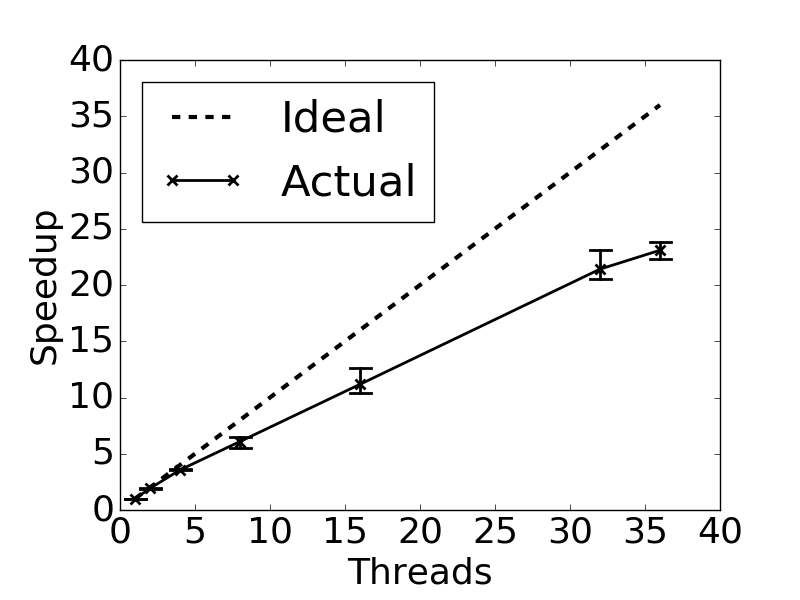
\includegraphics[width=\linewidth]{figures/results/performance/ls-parallel-scaling-tracks.png}
		\caption{By Tracks}
		\label{fig:rt-parallel-ls-tracks}
	\end{subfigure}
	\begin{subfigure}{0.48\textwidth}
		\centering
		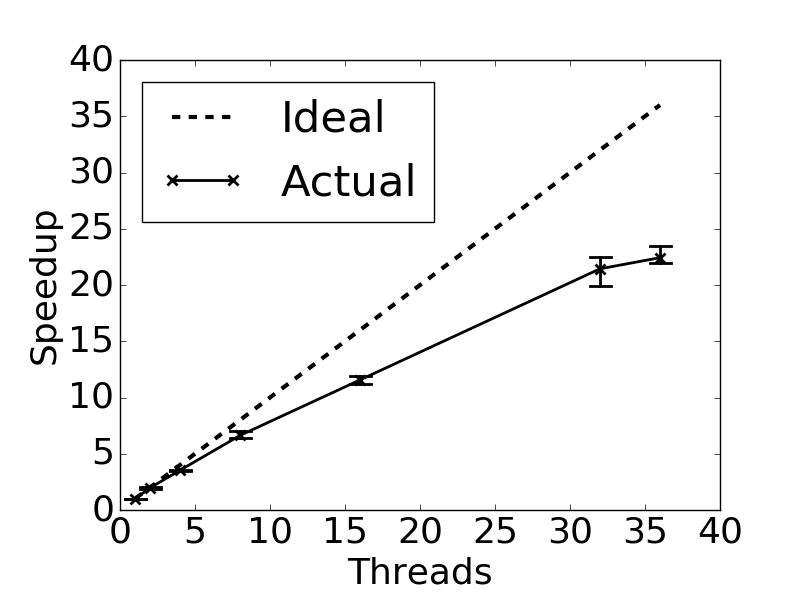
\includegraphics[width=\linewidth]{figures/results/performance/ls-parallel-scaling-stacks.png}
		\caption{By $Z$-Stacks}
		\label{fig:rt-parallel-ls-stacks}
	\end{subfigure}
	\caption[]{Strong scaling performance on the SDSA test problem using the Falcon supercomputer with on-the-fly ray tracing by (a) tracks and (b) $z$-stacks, both using the linear source \ac{MOC} solver.}
	\label{fig:rt-parallel-ls}
\end{figure}

As mentioned in the flat source ray tracing comparison,  performance using the full available resources is more important than single thread performance or scalability. Therefore, a comparison using full available resources on the Falcon supercomputer is is shown in Table~\ref{tab:rt-full-thread-ls}, showing again that ray tracing by $z$-stack seems to have slightly better performance than ray tracing by individual 3D track.

\begin{table}[ht]
	\centering
	\caption{Performance of the linear source solver on the SDSA test problem using full computational resources of a single Falcon node with 36 cores}
	\medskip
	\begin{tabular}{l|l|l}
		\hline
		Ray Tracing Scheme & Transport Sweep Time (s) & Integration Time (ns) \\
		\hline
		By Track & 103.3 +/- 3.4 & 1.33 +/- 0.06 \\
		By $z$-Stack & 101.2 +/- 4.4 & 1.36 +/- 0.05 \\
		\hline
	\end{tabular}
	\label{tab:rt-full-thread-ls}
\end{table}

\subsubsection{Performance on Cetus}

Lastly, performance tests of the ray tracing methods are conducted on the Cetus partition of the Argonne BlueGene/Q supercomputer, the targeted computer architecture for this thesis. Again, the same coarse ray parameters used in the flat source tests, and presented in Table~\ref{tab:rt-cetus-params}, are used for the linear source tests. Recall that while the BlueGene/Q architecture only has 16 CPU cores per node, the hyper-threads allow for improved resource utilization with up to 64 threads. The results are shown in Table~\ref{tab:rt-full-thread-cetus-ls}

\begin{table}[ht]
	\centering
	\caption{Performance on the SDSA test problem using full computational resources of a single Cetus node with 16 cores}
	\medskip
	\begin{tabular}{l|l|l}
		\hline
		Ray Tracing Scheme & Transport Sweep Time (s) & Integration Time (ns) \\
		\hline
		By Track & 31.88 +/- 0.52 & 11.00 +/- 0.18 \\
		By $z$-Stack & 31.68 +/- 0.26 & 10.93 +/- 0.09 \\
		\hline
	\end{tabular}
	\label{tab:rt-full-thread-cetus-ls}
\end{table}

These results again confirm that on-the-fly ray tracing by $z$-stack performs slightly better than on-the-fly ray tracing by individual 3D track. The scaling results with on-the-fly ray tracing by $z$-stack are shown in Figure~\ref{fig:rt-parallel-ls-cetus}. When 16 threads are used, in which the number of threads equals in the number of cores, the speedup is 90.9\% of idea. When all 64 available hyper-threads are utilized, the average speedup is 37.8, showing that latency is a major contributor to overall run-time and hyper-threads help alleviate these bottlenecks.

\begin{figure}[ht!]
	\centering
	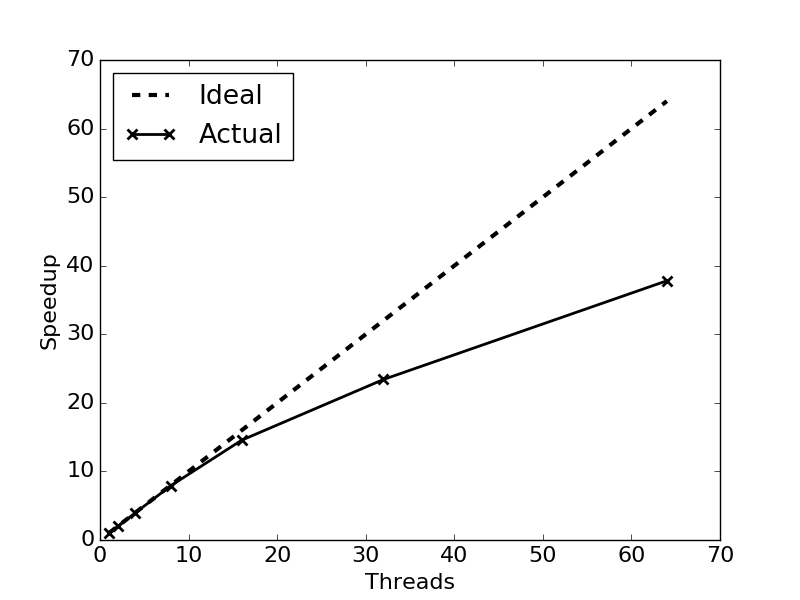
\includegraphics[width=0.75\linewidth]{figures/results/performance/ls-parallel-scaling-stacks-cetus.png}
	\caption{Strong scaling performance of the linear source solver on the SDSA test problem using the Cetus partition of the Argonne BlueGene/Q supercomputer with on-the-fly ray tracing by $z$-stacks.}
	\label{fig:rt-parallel-ls-cetus}
\end{figure}


\section{Conclusion}
\label{sec:ls-conclusion}



%\clearpage

\vfill
\begin{highlightsbox}[frametitle=Highlights]
\begin{itemize}
  \item A series of six 2D heterogeneous benchmark models were derived from the full core \ac{BEAVRS} model to explore spatial self-shielding effects on \ac{MGXS}.
  \item The benchmarks include individual fuel assemblies with different \ac{CRGT} and \ac{BP} configurations, 2$\times$2 fuel assembly colorsets with and without a water reflector, and the quarter core \ac{BEAVRS} model.
  \item The Shannon entropy was computed to determine the number of inactive batches needed when modeling each benchmark with OpenMC.
  \item Reference results for the eigenvalues, pin-wise fission rates and pin-wise U-238 capture rates were computed using OpenMC.
  \item The benchmarks and reference results are used in the following chapters to validate the use of statistical clustering methods to capture spatial self-shielding effects in \ac{MGXS} generated by OpenMC for OpenMOC.
\end{itemize}
\end{highlightsbox}
\vfill